\documentclass[10pt,aspectratio=169]{beamer}
\PassOptionsToPackage{table}{xcolor}
\usetheme{Warsaw}
\usepackage{lmodern}
\usepackage[sfdefault,light,lining]{FiraSans}
\usepackage{graphicx,amsmath,amssymb,booktabs,tikz}
\usetikzlibrary{positioning,arrows.meta}
\usepackage{tabularx}

\definecolor{headergray}{gray}{0.75}
\definecolor{rowgray}{gray}{0.92}

% --- Style Guide Colors [cite: 1] ---
\definecolor{LogicBlue}{RGB}{204,0,0}
\definecolor{InferenceRed}{RGB}{212,55,59}
\definecolor{LiteRed}{RGB}{248,232,232}

\setbeamercolor{structure}{fg=InferenceRed}
\setbeamercolor{frametitle}{bg=LogicBlue,fg=white}
\setbeamercolor{palette primary}{bg=LogicBlue,fg=white}
\setbeamercolor{palette secondary}{bg=InferenceRed,fg=white}
\setbeamercolor{block title}{bg=LogicBlue,fg=white}
\setbeamercolor{block body}{bg=LiteRed,fg=black}

\setbeamertemplate{navigation symbols}{}



% --- QR Code Logic [cite: 2, 3] ---
\addtobeamertemplate{frametitle}{}{
  \begin{tikzpicture}[remember picture,overlay]
    \ifnum\insertframenumber>1
      \node[anchor=north east, xshift=0mm, yshift=2mm] 
        at (current page.north east) 
        {
\includegraphics[width=20mm]{qrcode.png}};
    \fi
  \end{tikzpicture}
}
% --- Page Numbering m/n Bottom Right [cite: 1] ---
\setbeamerfont{page number in head/foot}{size=\large}
\setbeamertemplate{footline}{
  \ifnum\insertframenumber>1
    \hfill
    \vbox{
      \vspace{-1cm}
      \hbox{\usebeamercolor[fg]{page number in head/foot}
            \usebeamerfont{page number in head/foot}
            \insertframenumber\,/\,\inserttotalframenumber\kern1em}
    }
  \fi
}
\title{Is Hyper-Parameter Optimization Different for SE?}
\subtitle{Yes. And here's the math to prove it.}
\author{Rahul Yedida (Lexis Nexis) \and Tim Menzies (NCSU)}
\institute{\footnotesize NC State University, USA\\
timm@ieee.org
 \\ \url{http://timm.fyi} \\~\\ 
{\bf TSE}, 51(6), 2025, https://ieeexplore.ieee.org/document/10919477  \\
{\bf SLIDES}:
http://timm.fyi/26smooth.pdf
}

\date{Apr 17, 2026}

\begin{document}

\begin{frame}
\titlepage
\end{frame}
\newcommand{\yell}[1]{\color{red}{\bf #1}\color{black}}
\begin{frame}{Motivation: Off-the-Shelf AI for SE Data}

\begin{minipage}{0.66\textwidth}
    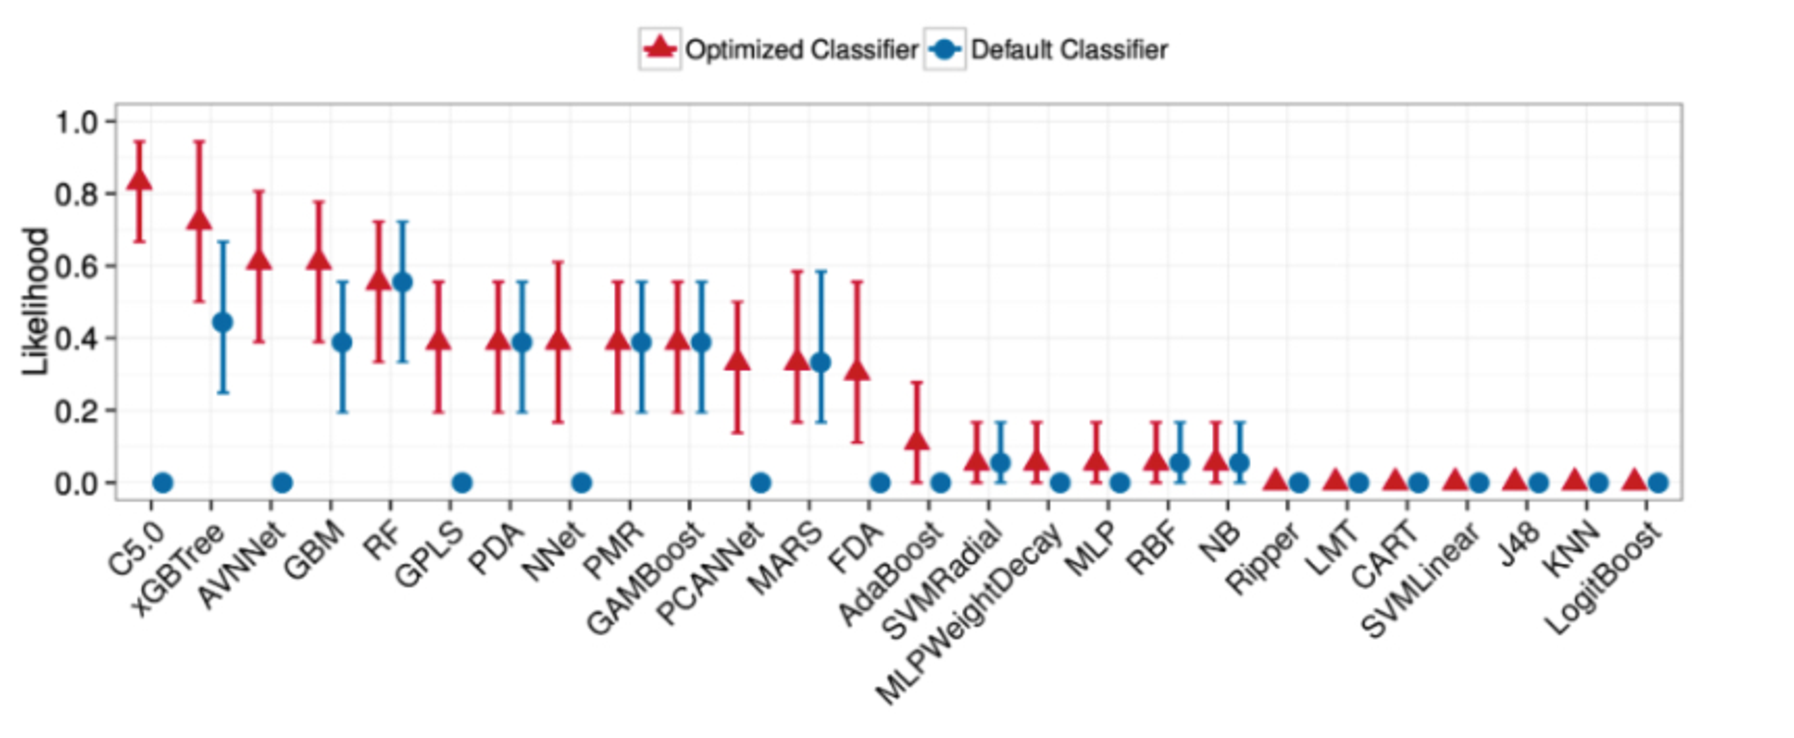
\includegraphics[height=1.5in]{tree.pdf}
\end{minipage}
\begin{minipage}{0.28\textwidth}
    \vspace{0pt} % ensures vertical alignment
    \raggedright
  \footnotesize    [Tantithamthavorn et al., ICSE'16]
\end{minipage}


Most SE research uses AI defaults without \yell{audit}.
\vspace{3mm}
\begin{itemize}
\item HPO = hyperparameter optimization. Black art of selecting tuning parameters.
\item HPO is applied to defect prediction and issue triage.
\item Current tools (NSGA-II, MOEA/D, SMAC3, BOHB, DEHB, etc) target \yell{general AI data}.
\item Question: Is SE data different? Does it need different kinds of learning?
\end{itemize}
\end{frame}

\begin{frame}{Message}
	\begin{center}
		
\includegraphics[height=2in]{head.jpg}
	\end{center}
	\begin{itemize}
\item All you LLM users-- you are missing what \yell{matters}.
\item SE-AI $\neq$ standard AI.
\item And you can \yell{leverage}~that.
	\end{itemize}
\end{frame}

\begin{frame}{So... many... studies....}
  \begin{columns}[T]
    \begin{column}{0.4\textwidth}
        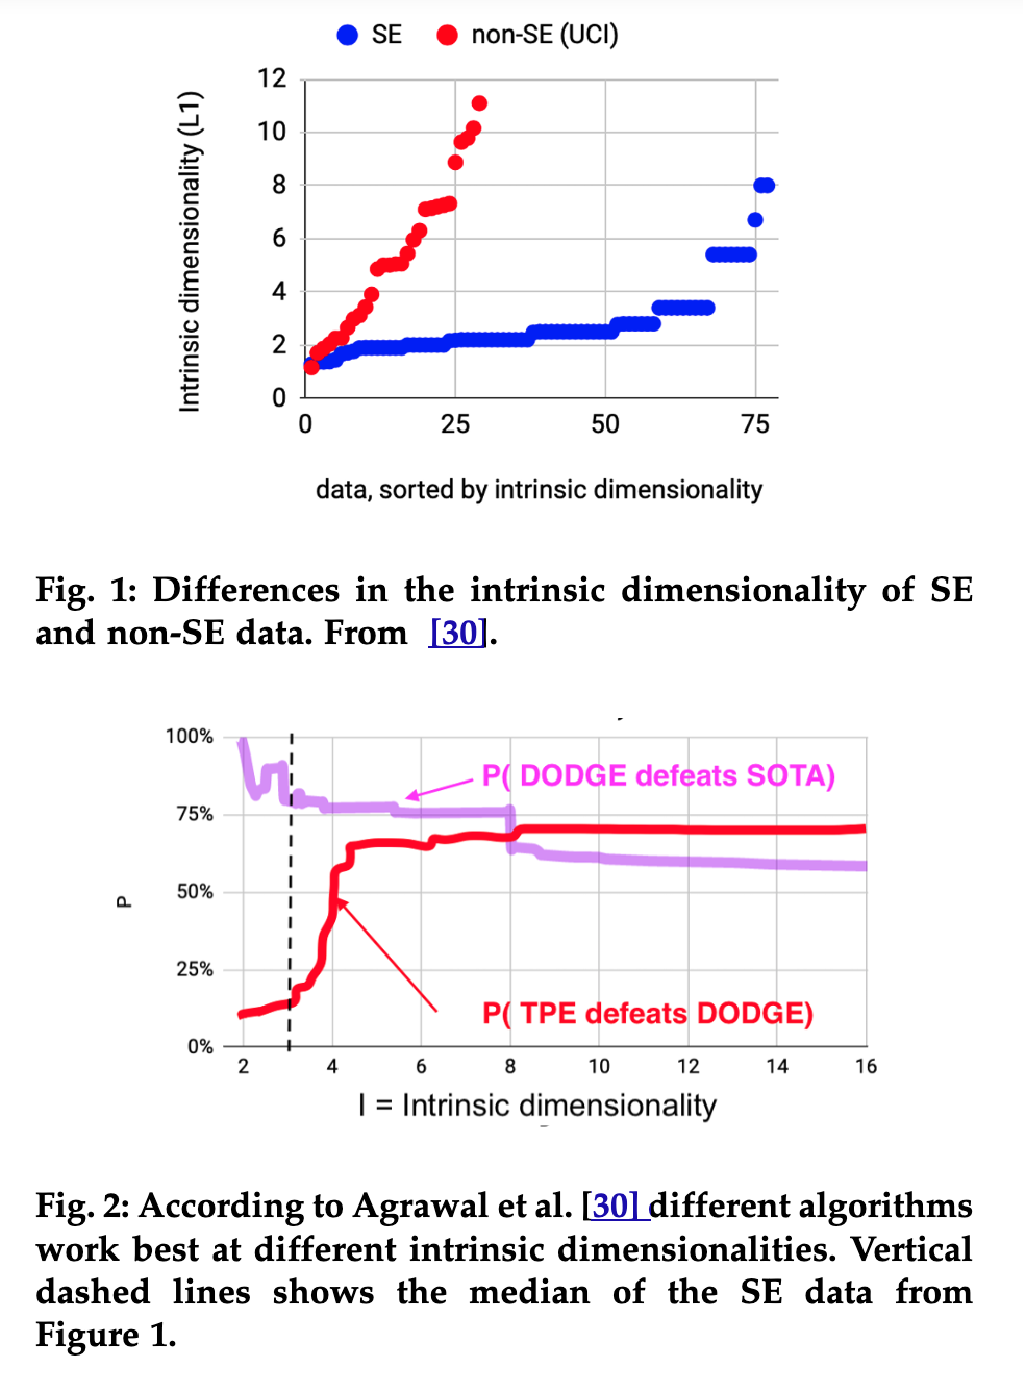
\includegraphics[height=3in]{ir.pdf}
    \end{column}
    \begin{column}{0.6\textwidth}
      \begin{itemize}
        \item 2021: Intrinsic dimensionality\\
              {\footnotesize \yell{doi.org/10.1109/TSE.2021.3073242}}
        \item DRR (data reduction ratio): 
                \begin{itemize} \item SE data ``flattens'' more than other data.\end{itemize}
        \item Count neighbors at $R_1$ vs.\ $n \times R_1$.
      \begin{itemize}
        \item Selects \yell{very simple} optimization problems.
        \item Most SE data sets are simple this way.
      \end{itemize}
\item \yell{Issue}:  not enough data to generalize
      \end{itemize}
    \end{column}
  \end{columns}
\end{frame}

\begin{frame}{So... many... (more) studies....}
  \begin{columns}[T]
    \begin{column}{0.57\textwidth}
      \begin{center}
        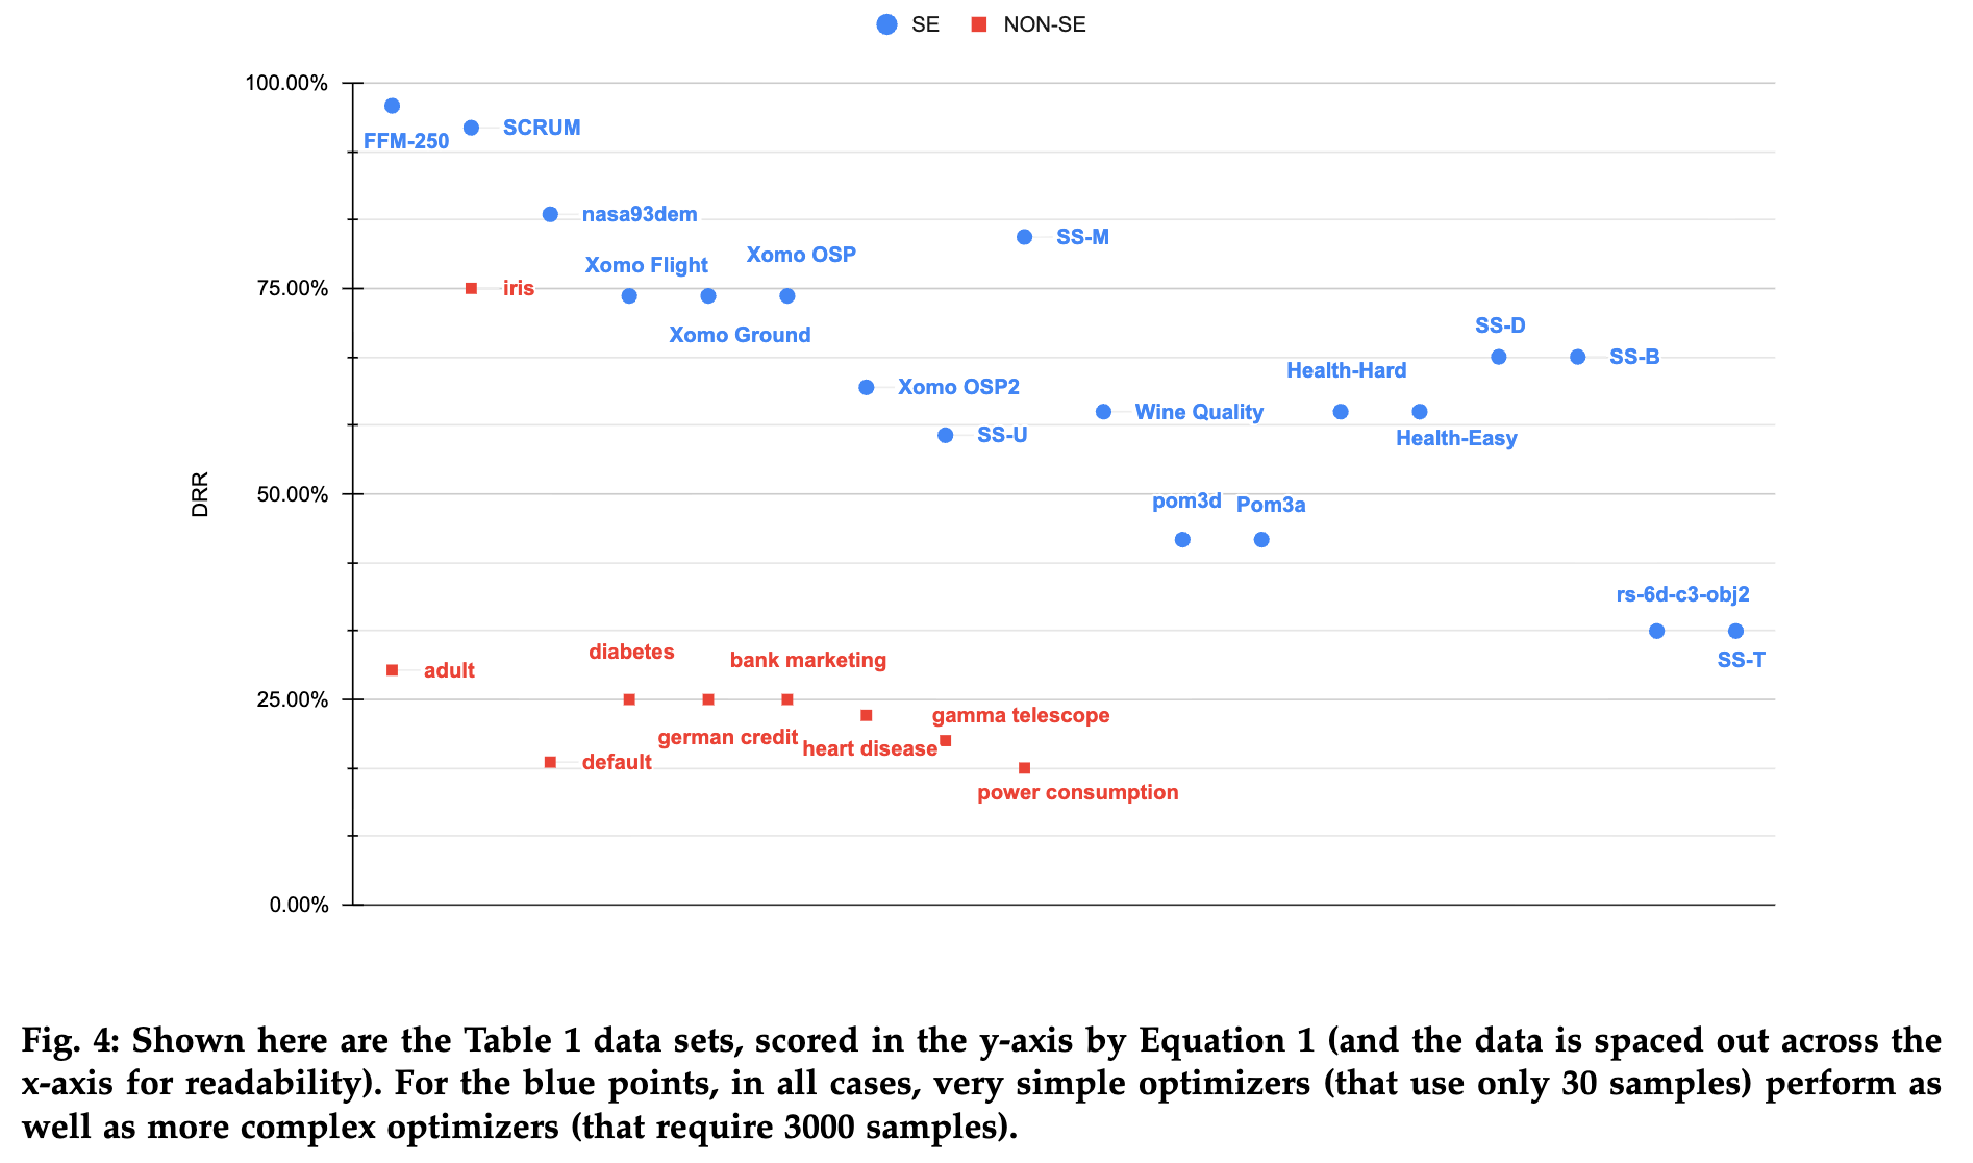
\includegraphics[height=2.1in]{drr.pdf}
      \end{center}
    \end{column}
    \begin{column}{0.43\textwidth}
      \begin{itemize}
        \item 2024: DRR (data reduction ratio)\\
              {\footnotesize \yell{arxiv.org/abs/2503.21086}}
        \item SE data ``flattens'' more than other data.
        \item Above the ``Andre threshold'', astonishingly simple methods work \yell{well}:
          \begin{itemize}
            \item Configuration
            \item Project management
            \item Hyperparameter optimization for \yell{predicting}~OSS project health
            \item Banking, health, power;
\item  etc.
          \end{itemize}
\item \yell{Issue}:  could not  explain "why"
      \end{itemize}
    \end{column}
  \end{columns}
\end{frame}

\begin{frame}{So ... many... (yet more).... studies...}
  \begin{columns}[T]
    \begin{column}{0.5\textwidth}
      \vspace{0pt}
      \begin{center}
        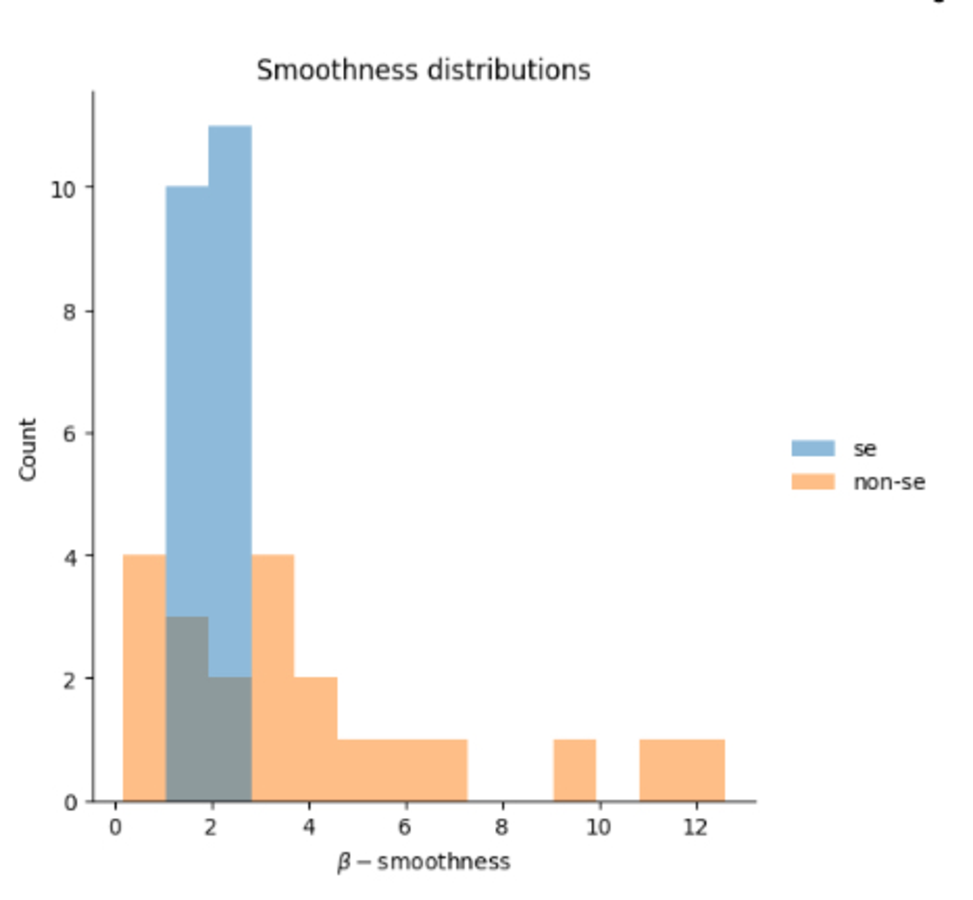
\includegraphics[height=2.8in]{senonse.pdf}
      \end{center}
    \end{column}
    \begin{column}{0.5\textwidth}
      \begin{itemize}
        \item 2025: this study
          \begin{itemize}
            \item SE data has ``smoother'' \yell{boundaries} between classes.
            \item Vs.\ AI data, magnitude of 2nd derivative of loss is much \yell{smaller}.
            \item Better HPO via \yell{AI designed for SE}.
          \end{itemize} ~\\
        \item 2026: FSE'26: BINGO effect\\
              {\footnotesize \yell{arxiv.org/pdf/2512.13524}}
          \begin{itemize}
            \item An even greater simplification.
          \end{itemize}~\\
        \item 2027: \yell{Rashomon}~sets (work in progress)
          \begin{itemize}
            \item Potentially: an end to hyperparameter optimization
          \end{itemize}
      \end{itemize}
    \end{column}
  \end{columns}
\end{frame}


\begin{frame}{The Observation: SE Loss Landscapes are Smoother}
  \textbf{Claim:} SE model loss landscapes are \yell{exploitably}~  smooth.
  ~\\
  \begin{center}
    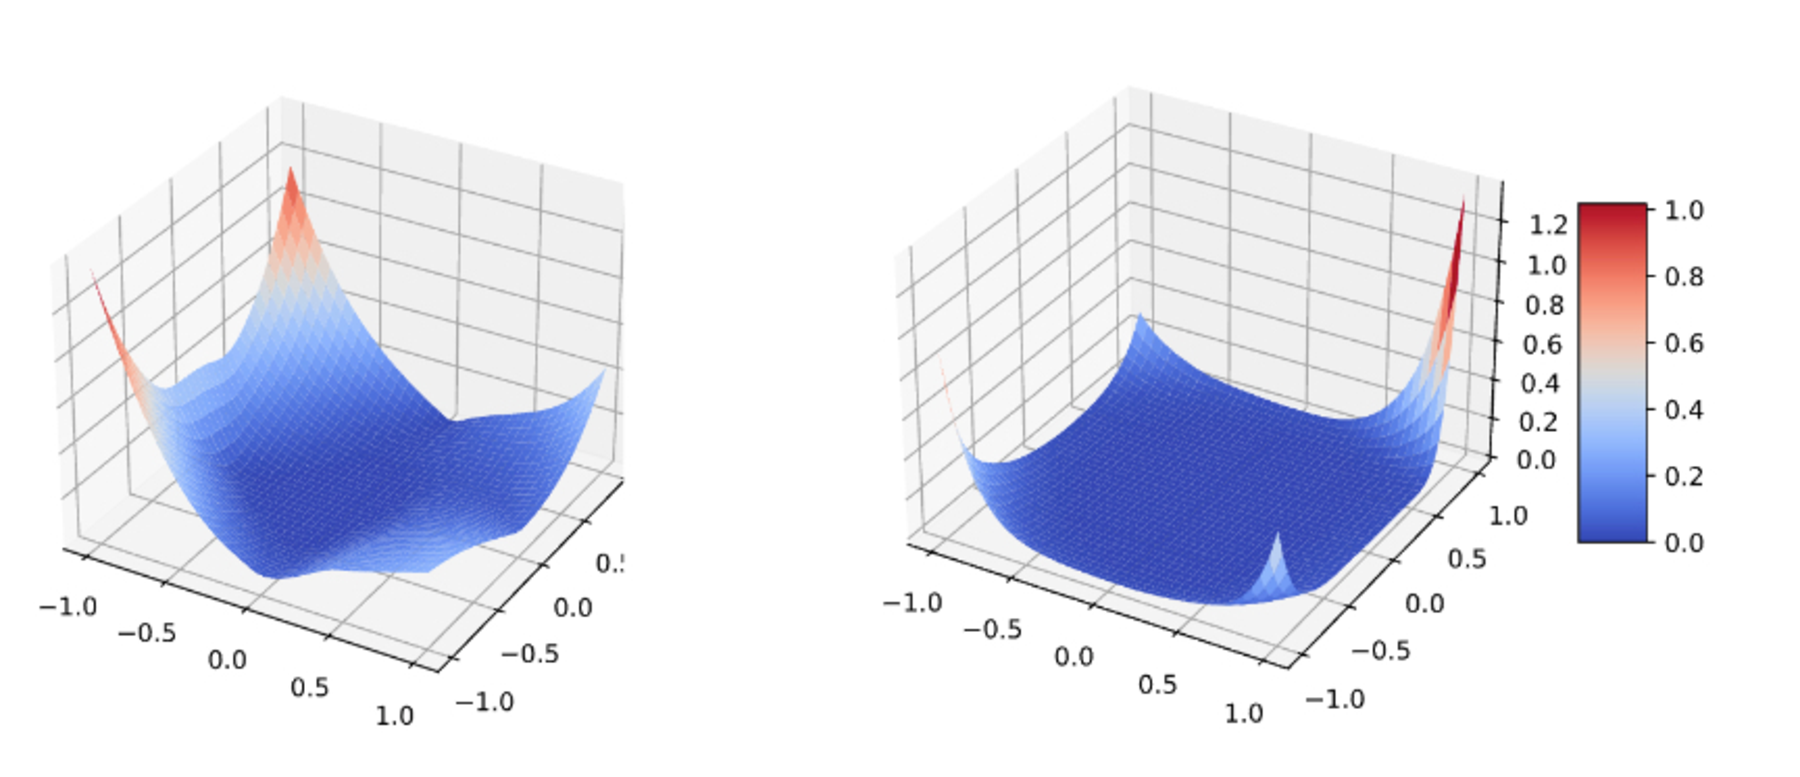
\includegraphics[height=1.5in]{hpo.pdf}
  \end{center}
  \vspace{1mm}
  \begin{block}{What ``smooth'' means (formally)}
    $f$ is $\beta$-smooth if: $\frac{\|\nabla f(y) - \nabla f(x)\|}{\|y - x\|} 
    \leq \beta$.
  \end{block}
  \vspace{3mm}
  \begin{itemize}
    \item SE data: mean $\beta$-smoothness $\approx$ 2.
    \item Standard AI (UCI) data: mean $\beta$-smoothness $\approx$ 5.
  \end{itemize}
\end{frame}

\begin{frame}{Why SE Data is Smooth: The Naturalness Argument}
  \begin{itemize}
    \item Human code is surprisingly \yell{repetitive}~ [Hindle et al. ICSE'12]
    \item Maintainability forces repeated use of idioms and patterns.
    \item Repetition $\Rightarrow$ minimal variation between clusters.
    \item Minimal variation $\Rightarrow$ flat loss \yell{landscapes}.
  \end{itemize}
  ~\\
  \begin{minipage}[t]{2in}
    \begin{block}{The core insight}
      Maintainable code produces data with flat loss landscapes.
    \end{block}\end{minipage}\hspace{1in}\begin{minipage}[t]{2in}
      \begin{block}{Effects of HPO}
        Smoothing the landscape.
      \end{block}\end{minipage}
    \end{frame}

    \begin{frame}[t]{Experiments with Hyper-parameters (not an exhaustive list)} 

    ~\\
\scriptsize
\begin{columns}[t]
\begin{column}{0.5\textwidth}
\begin{block}{\small Pre-processing (Basic)}
\begin{description}
\item[Normalization:] $x \rightarrow \frac{x}{\|x\|}$
\item[Standardization:] $x \rightarrow \frac{x - \mu_x}{\sigma_x}$
\item[Min-max scaling:] $x \rightarrow \frac{x - \min x}{\max x - \min x}$
\item[Max-abs scaling:] $x \rightarrow \frac{x}{\max |x|}$
\item[Robust scaling:] $x \rightarrow \frac{x - P_{50}(x)}{P_{75}(x) - P_{25}(x)}$
\end{description}
\end{block}

\vspace{1mm}

\begin{block}{\small Pre-processing (Advanced)}
\begin{description}
\item[SMOTE:] Synthetic minority samples via interpolation.
\item[Fuzzy sampling:] Allocates samples across layers ($\frac{1}{2^i}$) to rebalance.
\item[Semi-supervised labeling:] Label deletion and k-NN rebuild.
\end{description}
\end{block}
\end{column}


\begin{column}{0.5\textwidth}
\begin{block}{\small Neural Networks}
\begin{description}
\item[Feedforward:] 3--20 layers, 2--6 units/layer.
\item[Deep Learners:] More control parameters, e.g., topology, activation functions.
\end{description}
\end{block}

\vspace{1mm}

\begin{block}{\small Traditional Classifiers}
\begin{description}
\item[Neighbor classifiers:] (a) Distance measure, (b) neighbor count ($k$), (c) combination method, (d) pre-clustering.
\item[Random forests:] Number of trees, features per tree, polling method (majority or weighted).
\item[Logistic regression:] (a) Regularization type (L1, L2, elastic net), (b) strength ($C \in \{0.1, 1, 10\}$).
\end{description}
\end{block}
\end{column}
\end{columns}
\end{frame}

\begin{frame}{The Archive: 23 Datasets across 30 Years}
  \begin{minipage}[t]{0.4\textwidth}
\small
\begin{tabular}{lrrr}
\toprule
\textbf{Dataset} & \textbf{\#Trn} & \textbf{\#Tst} & \textbf{Feat} \\
\midrule
\textit{Defect prediction}  & & &  \\
camel    & 1819 & 442 & 20 \\
ivy      & 352  & 352 & 20 \\
log4j    & 244  & 205 & 20 \\
synapse  & 379  & 256 & 20 \\
velocity & 410  & 229 & 20 \\
xalan    & 2411 & 909 & 20 \\
\midrule
\textit{Static code warnings}  & & & \\
ant         & 28  & 7  & 329 \\
cassandra   & 13  & 4  & 265 \\
commons     & 17  & 5  & 127 \\
derby       & 366 & 92 & 292 \\
jmeter      & 14  & 4  & 287 \\
lucene-solr & 24  & 6  & 278 \\
tomcat      & 147 & 37 & 284 \\
\bottomrule
\end{tabular}
\end{minipage}
  \hspace{1cm}
  \begin{minipage}[t]{0.4\textwidth}
\small
\begin{tabular}{lrrr}
\toprule
\textbf{Dataset} & \textbf{\#Trn} & \textbf{\#Tst} & \textbf{Feat} \\
\midrule
\textit{Issue Lifetime Prediction }  & & &  \\
Eclipse  & 44545 & 25459 & 12 \\
Firefox  & 44800 & 25201 & 12 \\
Chromium & 44801 & 25200 & 12 \\
\midrule
  \textit{Bayesmark (from NuerIPS'20)} & & &  \\
breast   & 455  & 114 & 30 \\
digits   & 1438 & 359 & 64 \\
iris     & 120  & 30  & 4  \\
wine     & 142  & 36  & 13 \\
diabetes & 354  & 88  & 10 \\
\bottomrule
\end{tabular}
\end{minipage}
\end{frame}


\begin{frame}{The Algorithm: SMOOTHIE}
\centering
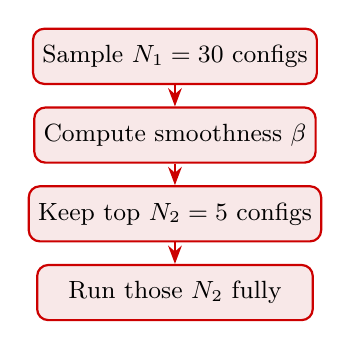
\begin{tikzpicture}[
box/.style={draw=LogicBlue, rounded corners, thick, fill=LiteRed,
minimum width=3.5cm, minimum height=0.7cm, font=\small},
line/.style={draw=LogicBlue, thick, -Stealth}]
\node[box] (s1) at (0,0) {Sample $N_1=30$ configs};
\node[box] (s2) at (0,-1) {Compute smoothness $\beta$};
\node[box] (s3) at (0,-2) {Keep top $N_2=5$ configs};
\node[box] (s4) at (0,-3) {Run those $N_2$ fully};
\draw[line] (s1)--(s2); \draw[line] (s2)--(s3); \draw[line] (s3)--(s4);
\end{tikzpicture}

\end{frame}

\begin{frame}{Finding 1 (RQ1): SMOOTHIE Wins on SE Data}
\begin{itemize}
\item \textbf{Static warnings:} SMOOTHIE \yell{wins}~4, ties 3.
\item \textbf{Issue lifetime:} Ties best in all 3 datasets.
\item \textbf{Defect prediction:} All methods tie (low \yell{complexity}).
\item \textbf{Data from AI:} On NuerIPS challenge data, no win.
\end{itemize}
\begin{block}{RQ1 Answer}
SMOOTHIE outperforms or matches SOTA on SE-specific data.
\end{block}
\begin{center}
  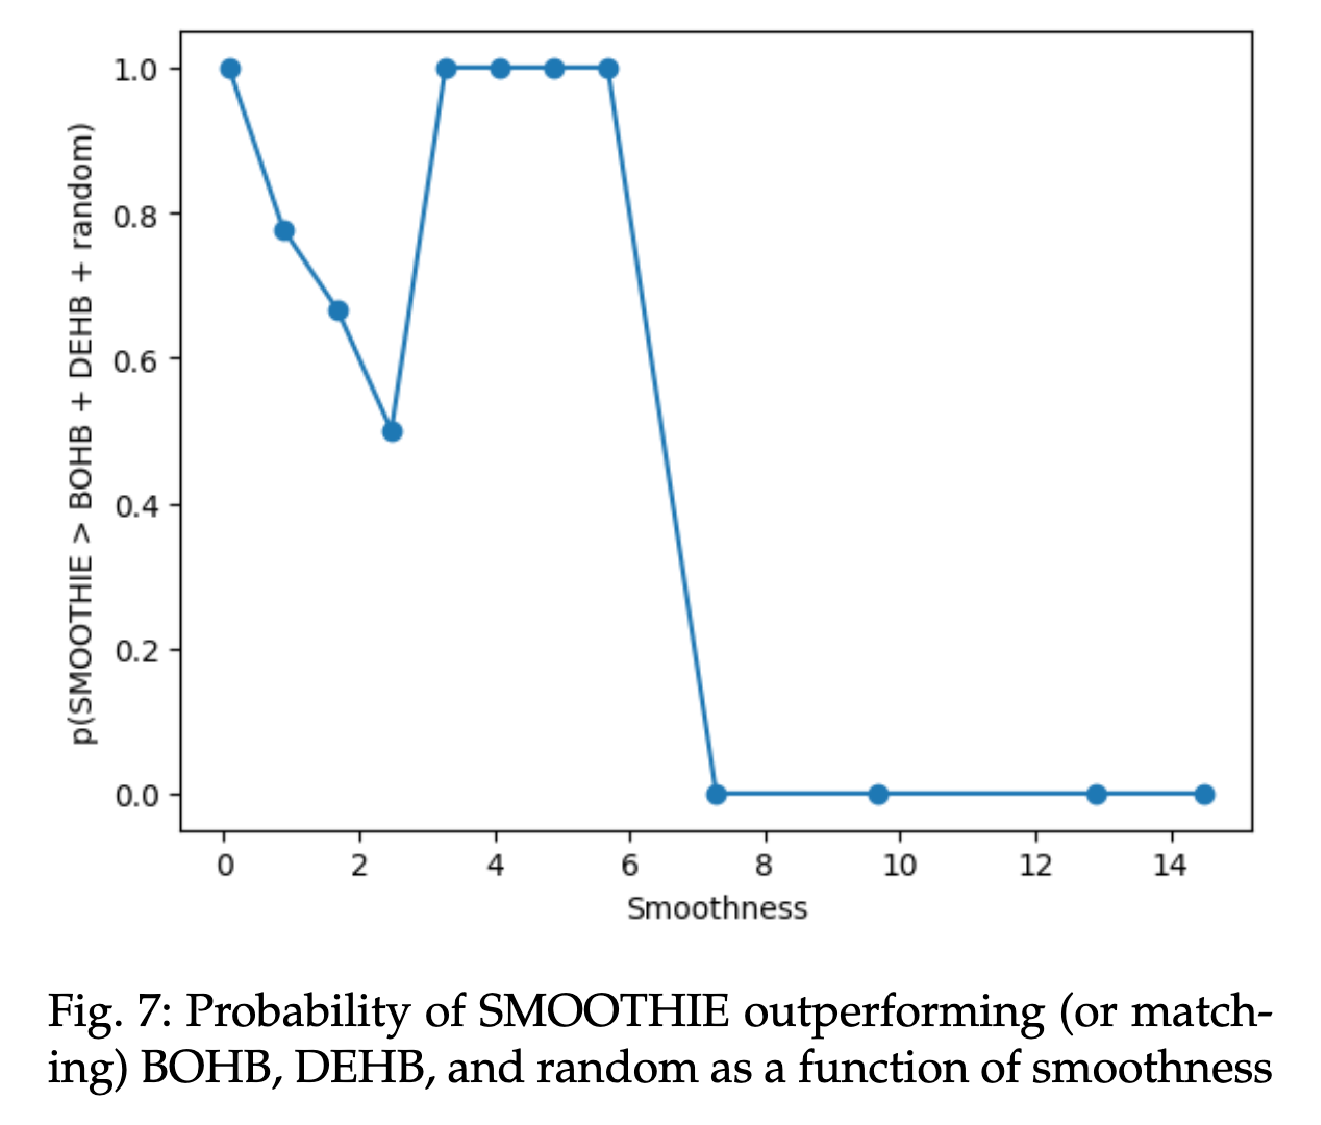
\includegraphics[height=2in]{prob.pdf}
\end{center}

\end{frame}

\begin{frame}{Finding 2 (RQ2): SMOOTHIE is Much Faster}
\begin{itemize}
\item Computing $\beta$ (Get-Smoothness) is \yell{negligible}.
\item End-to-end, SMOOTHIE is 4.7$\times$ faster than BOHB.
\item End-to-end, SMOOTHIE is 8.3$\times$ \yell{faster}~ than DEHB.
\end{itemize}
\begin{block}{RQ2 Answer}
SMOOTHIE achieves SOTA accuracy 4--8$\times$ faster.
\end{block}
\end{frame}

\begin{frame}{The End}
	\begin{center}
		
\includegraphics[height=2in]{head.jpg}
	\end{center}
	\begin{itemize}
\item All you LLM users-- you are missing what \yell{matters}.
\item SE-AI $\neq$ standard AI.
\item And you can \yell{leverage}~that.
\item Questions? Comments?
	\end{itemize}
\end{frame}


\end{document}
